\documentclass[a4paper]{report}
\usepackage[utf8]{inputenc}
\usepackage[T1]{fontenc}
\usepackage{RJournal}
\usepackage{amsmath,amssymb,array}
\usepackage{booktabs}
\usepackage{textcomp}

%!\SweaveUTF8
%\VignetteIndexEntry{ Measurement units in R }

\usepackage{Sweave}
\begin{document}

%% do not edit, for illustration only
\sectionhead{Contributed research article}
\volume{XX}
\volnumber{YY}
\year{20ZZ}
\month{AAAA}

%% replace RJtemplate with your article
\begin{article}
\title{Measurement units in R}
\author{Edzer Pebesma, Thomas Mailund, James Hiebert }

\maketitle

\abstract{ We briefly review SI units, and discuss R packages that
deal with measurement units, their compatibility and conversion.
Built upon \CRANpkg{udunits2} and the UNIDATA udunits library,
we introduce the package \CRANpkg{units} that provides a class for
maintaining unit metadata. When used in expression, it automatically
converts units, and simplifies units of results when possible; in
case of incompatible units, errors are raised. The class flexibly
allows expansion beyond predefined units.  Using \CRANpkg{units}
may eliminate a whole class of potential scientific programming
mistakes.  We discuss the potential and limitations of computing
with explicit units.  }


\section{Introduction}

Two quotes from \cite{cobb} -- {\em ``Data are not just numbers,
they are numbers with a context''} and  {\em ``in data analysis,
context provides meaning''} -- illustrate that for a data analysis
to be meaningful, knowledge of the data's context is needed.
Pragmatic aspects of this context include who collected or generated
the data, how this was done, and for which purpose \citep{scheider};
semantic aspects concern what the data represents: which aspect
of the world do the data refer to, when and where were they measured,
and what a value of \samp{1} means.

R does allow for keeping some context with data, for instance
\begin{itemize}
\item \code{"data.frame"} columns must have and \code{"list"} elements may have
names that can be used to describe context, using freetext
\item \code{"matrix"} or \code{"array"} objects may have \code{dimnames}
\item for variables of class \code{"factor"} or \code{"ordered"}, \code{levels}
may indicate, using freetext, the categories of nominal or ordinal variables
\item \code{"POSIXt"} and \code{"Date"} objects specify how numbers should
be interpreted as time or date, with fixed units (second and day, respectively)
and origin (Jan 1, 1970, 00:00 UTC)
\item \code{"difftime"} objects specify how time duration can be represented
by numbers, with flexible units (secs, mins, hours, days, weeks); \CRANpkg{lubridate}
\citep{lubridate} extends some of this functionality.
\end{itemize}
Furthermore, if spatial objects as defined in package \CRANpkg{sp}
\citep{sp} have a proper coordinate reference system set, they
can be transformed to other datums, or converted to various flat
(projected) representations of the Earth \citep{iliffe}.

In many cases however, R drops contextual information. As an example, we
look at annual global land-ocean temperature index\footnote{data from
\url{http://climate.nasa.gov/vital-signs/global-temperature/}} since 1960
(Fig \ref{fig}):
\begin{Schunk}
\begin{Sinput}
> temp_data = subset(read.table("647_Global_Temperature_Data_File.txt", 
+ 	header=TRUE)[1:2], Year >= 1960)
> temp_data$date = as.Date(paste0(temp_data$Year, "-01-01"))
> temp_data$time = as.POSIXct(temp_data$date)
> Sys.setenv(TZ="UTC")
> head(temp_data, 3)
\end{Sinput}
\begin{Soutput}
   Year Annual_Mean       date       time
81 1960       -0.03 1960-01-01 1960-01-01
82 1961        0.05 1961-01-01 1961-01-01
83 1962        0.02 1962-01-01 1962-01-01
\end{Soutput}
\begin{Sinput}
> year_duration = diff(temp_data$date)
> mean(year_duration)
\end{Sinput}
\begin{Soutput}
Time difference of 365.2545 days
\end{Soutput}
\end{Schunk}
\begin{figure}
\begin{center}
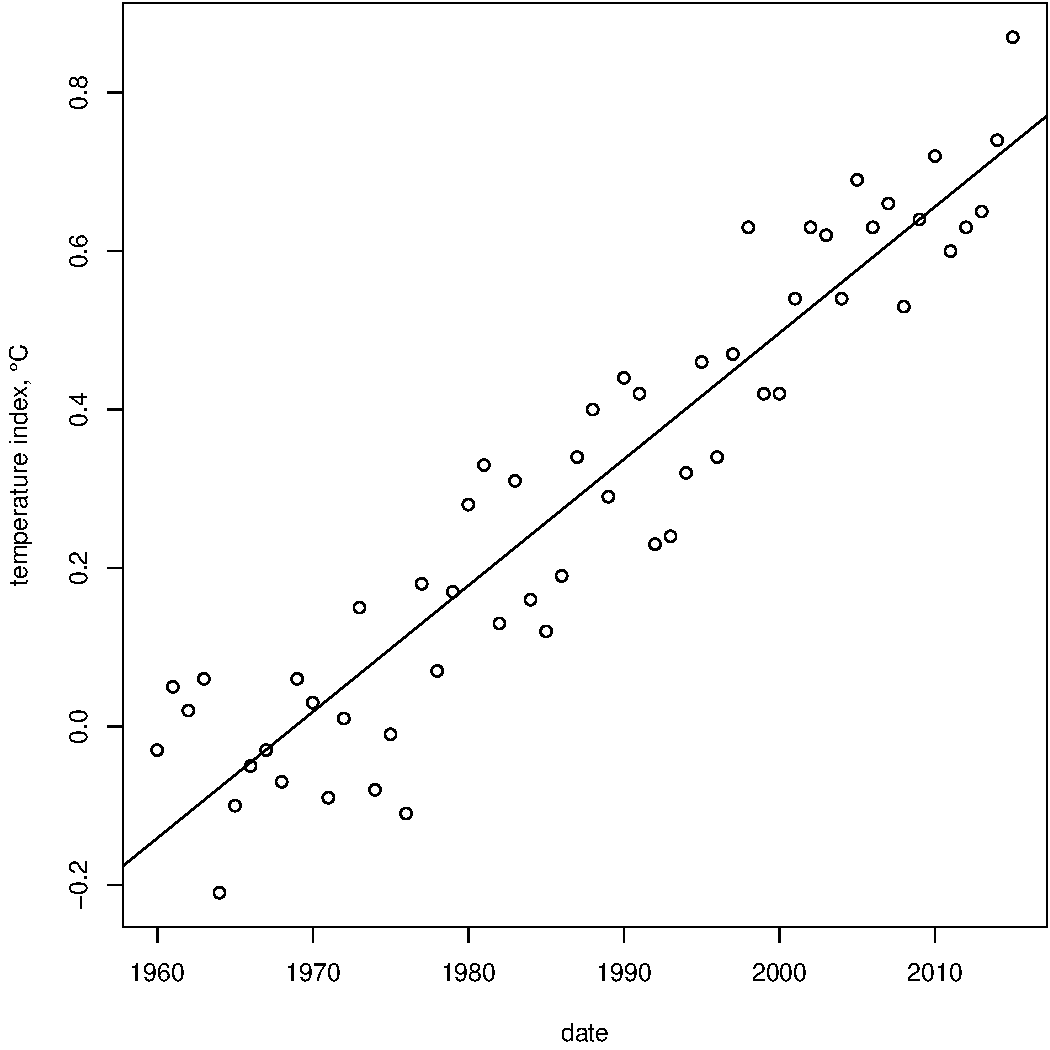
\includegraphics[scale=.5]{fig1}
\end{center}
\caption{Annual global land-ocean temperature index (\textdegree C), per year}
\label{fig}
\end{figure}
Here, the time difference units are reported for the \code{difftime} 
object \code{year\_duration}, but
if we would use it in a linear algebra operation
\begin{Schunk}
\begin{Sinput}
> year_duration %*% rep(1, length(year_duration)) / length(year_duration)
\end{Sinput}
\begin{Soutput}
         [,1]
[1,] 365.2545
\end{Soutput}
\end{Schunk}
the unit is dropped. Similarly, for linear regression coefficients we see
\begin{Schunk}
\begin{Sinput}
> coef(lm(Annual_Mean ~ date, temp_data))
\end{Sinput}
\begin{Soutput}
 (Intercept)         date 
1.833671e-02 4.364763e-05 
\end{Soutput}
\begin{Sinput}
> coef(lm(Annual_Mean ~ time, temp_data))
\end{Sinput}
\begin{Soutput}
 (Intercept)         time 
1.833671e-02 5.051809e-10 
\end{Soutput}
\end{Schunk}
where the unit of change is in degrees Celcius but either per day
(date) or per second (time). For purely mathematical manipulations,
R often strips context from numbers when it is carried in attributes,
the linear algebra routines being a prime example.

Most variables are somehow attributed with information about
their {\em units}, which specify what the value 1 of this variable
represents.  This may be counts of something, e.g. \samp{1 apple},
but it may also refer to some {\em physical unit}, such as distance
in meter. This article discusses how strong unit support can be
introduced in R.

\section{SI}

The BIPM (Bureau International des Poids et Mesures) is the
``{\em the intergovernmental organization through which Member
States act together on matters related to measurement science and
measurement standards.  Its recommended practical system of units
of measurement is the International System of Units (Syst\`{e}me
International d'Unit\'{e}s, with the international abbreviation
SI)}\footnote{\url{http://www.bipm.org/en/measurement-units/}}''.
\cite{si} describe the SI units, where, briefly, {\em SI units}
\begin{itemize}
\item consist of seven base units (length, mass, time \& duration,
electric current, thermodynamic temperature, amount of substance, and
luminous intensity), each with a name and abbreviation (Table \ref{tab:si})
\item consist of {\em derived units} that are formed by products of 
powers of base units, such as \samp{$m/s^2$}, many of which have special
names and symbols (e.g.~angle: 1 rad = 1 m/m; force: 1 N = 1 m kg s$^{-2}$)
\item consist of {\em coherent derived units} when derived units
include no numerical factors other than one (with the exception
of \samp{kg}\footnote{as a base unit, kg can be part of coherent derived units});
an example of a coherent derived unit is 1 watt = 1 joule per 1 second,
\item may contain SI prefixes (k = kilo for $10^3$, m = milli for $10^{-3}$, etc.)
\item contain special quantities where units disappear (e.g., m/m) or 
have the nature of a count, in which cases the unit is \samp{1}.
\end{itemize}

\begin{table}[bt]
\begin{center}
\begin{tabular}{llll}\hline
\multicolumn{2}{l}{Base quantity} & \multicolumn{2}{l}{SI base unit} \\\hline
Name & Symbol & Name & Symbol \\ \hline
length & $l,x,r,$ etc. & meter & m\\
mass & $m$ & kilogram & kg\\
time, duration & $t$ & second & s \\
electric current & $I, i$ & ampere & A \\
thermodynamic temperature & $T$ & kelvin & K \\
amount of substance & $n$ & mole & mol \\
luminous intensity & $I_v$ & candela & cd  \\\hline
\end{tabular}
\end{center}
\caption{base quantities, SI units and their symbols (from \cite{si}, p. 23)}
\label{tab:si}
\end{table}

\section{Related work in R}

Several R packages provide unit conversions. 
For instance, \CRANpkg{measurements} \citep{measurements} provides
a collection of tools to make working with physical measurements
easier. It converts between metric and imperial units, or calculates
a dimension's unknown value from other dimensions' measurements. It
does this by the \samp{conv\_unit} function:
\begin{Schunk}
\begin{Sinput}
> library(measurements)
> conv_unit(2.54, "cm", "inch")
\end{Sinput}
\begin{Soutput}
[1] 1
\end{Soutput}
\begin{Sinput}
> conv_unit(c("101 44.32","3 19.453"), "deg_dec_min", "deg_min_sec")
\end{Sinput}
\begin{Soutput}
[1] "101 44 19.2000000000116" "3 19 27.1800000000003"  
\end{Soutput}
\begin{Sinput}
> conv_unit(10, "cm_per_sec", "km_per_day")
\end{Sinput}
\begin{Soutput}
[1] 8.64
\end{Soutput}
\end{Schunk}
but uses for instance \code{kph} instead of \samp{km\_per\_hour}, and then
\samp{m3\_per\_hr} for flow -- unit names seem to come from convention rather
than systematic composition.  Object
\code{conv\_unit\_options} contains all 173 supported units, categorized by
(derived) unit:
\begin{Schunk}
\begin{Sinput}
> names(conv_unit_options)
\end{Sinput}
\begin{Soutput}
 [1] "acceleration" "angle"        "area"         "coordinate"   "count"       
 [6] "duration"     "energy"       "flow"         "length"       "mass"        
[11] "power"        "pressure"     "speed"        "temperature"  "volume"      
\end{Soutput}
\begin{Sinput}
> conv_unit_options$volume
\end{Sinput}
\begin{Soutput}
 [1] "ul"        "ml"        "dl"        "l"         "cm3"       "dm3"      
 [7] "m3"        "km3"       "us_tsp"    "us_tbsp"   "us_oz"     "us_cup"   
[13] "us_pint"   "us_quart"  "us_gal"    "inch3"     "ft3"       "mi3"      
[19] "imp_tsp"   "imp_tbsp"  "imp_oz"    "imp_cup"   "imp_pint"  "imp_quart"
[25] "imp_gal"  
\end{Soutput}
\end{Schunk}
Function \samp{conv\_dim} allows for the conversion of units in products or ratios,
e.g.
\begin{Schunk}
\begin{Sinput}
> conv_dim(x = 100, x_unit = "m", trans = 3, trans_unit = "ft_per_sec", y_unit = "min")
\end{Sinput}
\begin{Soutput}
[1] 1.822689
\end{Soutput}
\end{Schunk}
computes how many minutes it takes to travel 100 meters at 3 feet per second.

Package \CRANpkg{NISTunits} \citep{NISTunits} provides fundamental
physical constants (Quantity, Value, Uncertainty, Unit) for SI and
non-SI units, plus unit conversions, based on the data from NIST
(National Institute of Standards and Technology). The package
provides a single function for every
unit conversion; all but 5 from its 896 functions are of the form
\samp{NISTxxxTOyyy} where \samp{xxx} and \samp{yyy} refer to two
different units. For instance, converting from W m$^{-2}$ to W {\em inch}$^{-2}$
is done by
\begin{Schunk}
\begin{Sinput}
> library(NISTunits)
> NISTwattPerSqrMeterTOwattPerSqrInch(1:5)
\end{Sinput}
\begin{Soutput}
[1] 0.00064516 0.00129032 0.00193548 0.00258064 0.00322580
\end{Soutput}
\end{Schunk}
Both \CRANpkg{measurements} and \CRANpkg{NISTunits} are written entirely
in R.

\section{UNIDATA's udunits library and the \code{udunits2} R package}

Udunits, developed by UCAR/UNIDATA, advertises itself on its web
page\footnote{\url{https://www.unidata.ucar.edu/software/udunits/}}
as: ``{\em The udunits package supports units of physical
quantities. Its C library provides for arithmetic manipulation
of units and for conversion of numeric values between compatible
units. The package contains an extensive unit database, which is
in XML format and user-extendable.} The R package \CRANpkg{udunits2}
\citep{udunits2} provides an R level interface to the most important
functions in the C library.

The functions provided by \CRANpkg{udunits2} are
\begin{Schunk}
\begin{Sinput}
> library(udunits2)
> ls(2)
\end{Sinput}
\begin{Soutput}
[1] "ud.are.convertible"  "ud.convert"          "ud.get.name"        
[4] "ud.get.symbol"       "ud.have.unit.system" "ud.is.parseable"    
[7] "ud.set.encoding"    
\end{Soutput}
\end{Schunk}
Dropping the \samp{ud} prefix,
\samp{is.parseable} verifies whether a unit is parseable
\begin{Schunk}
\begin{Sinput}
> ud.is.parseable("m/s")
\end{Sinput}
\begin{Soutput}
[1] TRUE
\end{Soutput}
\begin{Sinput}
> ud.is.parseable("q")
\end{Sinput}
\begin{Soutput}
[1] FALSE
\end{Soutput}
\end{Schunk}
\samp{are.convertible} specifies whether two units are convertible
\begin{Schunk}
\begin{Sinput}
> ud.are.convertible("m/s", "km/h")
\end{Sinput}
\begin{Soutput}
[1] TRUE
\end{Soutput}
\begin{Sinput}
> ud.are.convertible("m/s", "s")
\end{Sinput}
\begin{Soutput}
[1] FALSE
\end{Soutput}
\end{Schunk}
\samp{convert} converts units that are convertible, and throws an error otherwise
\begin{Schunk}
\begin{Sinput}
> ud.convert(1:3, "m/s", "km/h")
\end{Sinput}
\begin{Soutput}
[1]  3.6  7.2 10.8
\end{Soutput}
\end{Schunk}
and \samp{get.name}, \samp{get.symbol} and \samp{set.encoding} get name, get symbol
or modify encoding of the character unit arguments.
\begin{Schunk}
\begin{Sinput}
> ud.get.name("kg")
\end{Sinput}
\begin{Soutput}
[1] "kilogram"
\end{Soutput}
\begin{Sinput}
> ud.get.symbol("kilogram")
\end{Sinput}
\begin{Soutput}
[1] "kg"
\end{Soutput}
\begin{Sinput}
> ud.set.encoding("utf8")
\end{Sinput}
\begin{Soutput}
NULL
\end{Soutput}
\end{Schunk}

Unlike the \CRANpkg{measurements} and \CRANpkg{NISTunits},
\CRANpkg{udunits2} parses units as expressions, and bases its logic
upon the convertibility of expressions, rather than the comparison of 
fixed strings:
\begin{Schunk}
\begin{Sinput}
> m100_a = paste(rep("m", 100), collapse = "*")
> m100_b = "dm^100"
> ud.is.parseable(m100_a)
\end{Sinput}
\begin{Soutput}
[1] TRUE
\end{Soutput}
\begin{Sinput}
> ud.is.parseable(m100_b)
\end{Sinput}
\begin{Soutput}
[1] TRUE
\end{Soutput}
\begin{Sinput}
> ud.are.convertible(m100_a, m100_b)
\end{Sinput}
\begin{Soutput}
[1] TRUE
\end{Soutput}
\end{Schunk}
This has the advantage that through complex computations,
intermediate objects can have units that are arbitrarily complex,
and that can potentially be simplified later on. It also means that
the package practically supports an unlimited amount of derived units.

\section{Udunits versus the Unified Code for Units of Measure (UCUM)}

Another set of encodings for measurement units is the Unified Code for
Units of Measure (UCUM, \cite{ucum}). A dedicated web
site\footnote{\url{http://coastwatch.pfeg.noaa.gov/erddap/convert/units.html}}
describes the details of the differences between udunits and UCUM,
and provides a conversion service between the two encoding sets. 

The UCUM website refers to some Java implementations, but some of the
links seem to be dead.  UCUM is the preferred encoding for standards
from the Open Geospatial Consortium. udunits on the other hand
is the units standard of choice by the climate science community,
and is adopted by the CF (Climate and Forecast) conventions, which
mostly uses NetCDF. NetCDF \citep{netcdf} is a binary data format
that is widely used for atmospheric and climate model predictions.

The udunits library is a C library that has strong support from
UNIDATA, and we decided to build our developments on this, rather
than on Java implementations of UCUM with a less clear provenance.

\section{Handling data with units in R: the \CRANpkg{units} package}

The \CRANpkg{units} package builds \code{"units"} objects from scratch,
where \samp{m}, created by
\begin{Schunk}
\begin{Sinput}
> library(units)
> m = make_unit("m")
> str(m)
\end{Sinput}
\begin{Soutput}
Class 'units'  atomic [1:1] 1
  ..- attr(*, "units")=List of 2
  .. ..$ numerator  : chr "m"
  .. ..$ denominator: chr(0) 
  .. ..- attr(*, "class")= chr "symbolic_units"
\end{Soutput}
\end{Schunk}
represents \samp{1 m}, one meter. Other length values are obtained by using this
unit in an expression:
\begin{Schunk}
\begin{Sinput}
> x1 = 1:5 * m
\end{Sinput}
\end{Schunk}
As an alternative to using \samp{make\_unit}, we can retrieve units directly
from the \samp{ud\_units} database, which is part of \CRANpkg{units}, and was
derived from the xml units database that is part of udunits. Two ways of doing
this are
\begin{Schunk}
\begin{Sinput}
> x2 = 1:5 * ud_units$m
> identical(x1, x2)
\end{Sinput}
\begin{Soutput}
[1] TRUE
\end{Soutput}
\begin{Sinput}
> x3 = 1:5 * with(ud_units, m)
> identical(x1, x3)
\end{Sinput}
\begin{Soutput}
[1] TRUE
\end{Soutput}
\end{Schunk}
Although one could attach \samp{ud\_units} to use the units directly,
there are over 3000 and this would not only clobber the namespace
but also lead to conflicts, e.g. for \samp{T} (Tesla, \code{TRUE})
or \samp{in} (inch, reserved R language element). The last form using
\samp{with} has the advantage that it can take direct expressions:
\begin{Schunk}
\begin{Sinput}
> with(ud_units, m/s^2)
\end{Sinput}
\begin{Soutput}
1 m/s^2
\end{Soutput}
\end{Schunk}
Several manipulations with \code{"units"} objects will now be illustrated.

\begin{Schunk}
\begin{Sinput}
> m =  with(ud_units,  m)
> km = with(ud_units, km)
> cm = with(ud_units, cm)
> s =  with(ud_units,  s)
> h =  with(ud_units,  h)
\end{Sinput}
\end{Schunk}

Manipulations that do not involve unit conversion are for instance addition:
\begin{Schunk}
\begin{Sinput}
> x = 1:3 * m/s
> x + 2 * x
\end{Sinput}
\begin{Soutput}
Units: m/s
[1] 3 6 9
\end{Soutput}
\end{Schunk}
Explicit unit conversion is done by assigning new units:
\begin{Schunk}
\begin{Sinput}
> units(x) = cm/s
> x
\end{Sinput}
\begin{Soutput}
Units: cm/s
[1] 100 200 300
\end{Soutput}
\begin{Sinput}
> as.numeric(x)
\end{Sinput}
\begin{Soutput}
[1] 100 200 300
\end{Soutput}
\end{Schunk}
similar to the behaviour of \code{"difftime"} objects, this modifies
the numeric values without modifying their meaning (what the numbers
refer to).

When mixing units in sums, comparisons or concatenation, units are 
automatically converted to those of the first argument:
\begin{Schunk}
\begin{Sinput}
> y = 1:3 * km/h
> x + y
\end{Sinput}
\begin{Soutput}
Units: cm/s
[1] 127.7778 255.5556 383.3333
\end{Soutput}
\begin{Sinput}
> y + x
\end{Sinput}
\begin{Soutput}
Units: km/h
[1]  4.6  9.2 13.8
\end{Soutput}
\begin{Sinput}
> x < y
\end{Sinput}
\begin{Soutput}
[1] FALSE FALSE FALSE
\end{Soutput}
\begin{Sinput}
> c(y, x)
\end{Sinput}
\begin{Soutput}
Units: km/h
[1]  1.0  2.0  3.0  3.6  7.2 10.8
\end{Soutput}
\end{Schunk}
where \code{c(y, x)} concatenates \code{y} and \code{x} after converting \code{x} to the
units of \code{y}. Derived units are created where appropriate:
\begin{Schunk}
\begin{Sinput}
> x * y
\end{Sinput}
\begin{Soutput}
Units: cm*km/h/s
[1] 100 400 900
\end{Soutput}
\begin{Sinput}
> x^3
\end{Sinput}
\begin{Soutput}
Units: cm^3/s^3
[1] 1.0e+06 8.0e+06 2.7e+07
\end{Soutput}
\end{Schunk}
and meaningful error messages appear when units are not compatible:
\begin{Schunk}
\begin{Sinput}
> e = try(z <- x + x * y)
> attr(e, "condition")[[1]]
\end{Sinput}
\begin{Soutput}
[1] "cannot convert cm*km/h/s into cm/s"
\end{Soutput}
\end{Schunk}
The full set of methods and method groups for \samp{units} objects is shown by
\begin{Schunk}
\begin{Sinput}
> methods(class = "units")
\end{Sinput}
\begin{Soutput}
 [1] as.data.frame c             diff          format        hist         
 [6] Math          mean          median        Ops           plot         
[11] print         quantile      Summary       [             units<-      
[16] units         weighted.mean
see '?methods' for accessing help and source code
\end{Soutput}
\end{Schunk}
where the method groups
\begin{itemize}
\item \code{Ops} include operations that require compatible units,
converting when necessary (\code{+}, \code{-}, \code{==}, \code{!=},
\code{<}, \code{>}, \code{<=}, \code{>=}), and operations that create
new units (\code{*}, \code{/}, \code{\^{}} and \code{**}),
\item \code{Math} include \code{abs}, \code{sign}, \code{floor},
\code{ceiling}, \code{trunc}, \code{round}, \code{signif}, \code{log},
\code{cumsum}, \code{cummax}, \code{cummin}, and
\item \code{Summary} include \code{sum}, \code{min}, \code{max} and \code{range},
and all convert to the unit of the first argument.
\end{itemize}
When possible, new units are simplified:
\begin{Schunk}
\begin{Sinput}
> a = 1:10 * m/s
> b = 1:10 * h
> a * b
\end{Sinput}
\begin{Soutput}
Units: m
 [1]   3600  14400  32400  57600  90000 129600 176400 230400 291600 360000
\end{Soutput}
\begin{Sinput}
> make_unit(m100_a) / make_unit(m100_b)
\end{Sinput}
\begin{Soutput}
1e+100 1
\end{Soutput}
\end{Schunk}

Units are printed as simple R expressions, but this looks odd in cases like
\begin{Schunk}
\begin{Sinput}
> m^5/s^4
\end{Sinput}
\begin{Soutput}
1 m^5/s^4
\end{Soutput}
\end{Schunk}
Another way to print units commonly seen in Climate and Forecast Conventions\footnote{CF, \url{http://cfconventions.org/Data/cf-standard-names/34/build/cf-standard-name-table.html}} is \samp{m2 s-1} for $m^2/s$. These are not R expressions, but as they are understood by udunits,
they can be converted (by udunits) but not simplified (by R):
\begin{Schunk}
\begin{Sinput}
> x = make_unit("m2 s-1")
> y = km^2/h
> z = m^2/s
> x + y
\end{Sinput}
\begin{Soutput}
278.7778 (m2 s-1)
\end{Soutput}
\begin{Sinput}
> x/y
\end{Sinput}
\begin{Soutput}
1 h*(m2 s-1)/km^2
\end{Soutput}
\begin{Sinput}
> z/y
\end{Sinput}
\begin{Soutput}
0.0036 1
\end{Soutput}
\end{Schunk}
However, \samp{parse\_unit} parses such units, and \samp{as\_cf} returns such unit strings from \code{"units"} objects:
\begin{Schunk}
\begin{Sinput}
> parse_unit("m2 s-1")
\end{Sinput}
\begin{Soutput}
1 m^2/s
\end{Soutput}
\begin{Sinput}
> as_cf(m^2*s^-1)
\end{Sinput}
\begin{Soutput}
[1] "m2 s-1"
\end{Soutput}
\end{Schunk}

Automatic conversion between \code{"units"} and \code{"difftime"} is provided: 
\begin{Schunk}
\begin{Sinput}
> (dt = diff(Sys.time() + c(0, 1, 1+60, 1+60+3600))) # class difftime
\end{Sinput}
\begin{Soutput}
Time differences in secs
[1]    1   60 3600
\end{Soutput}
\begin{Sinput}
> (dt.u = as.units(dt))
\end{Sinput}
\begin{Soutput}
Units: s
[1]    1   60 3600
\end{Soutput}
\begin{Sinput}
> identical(as.dt(dt.u), dt) # as.difftime is not a generic
\end{Sinput}
\begin{Soutput}
[1] TRUE
\end{Soutput}
\end{Schunk}
Objects of class \code{"units"} can be used as columns in \code{"data.frame"}
objects, as well as in \code{"tbl\_df"} \citep{tibble}.

\section{Discussion and conclusions}

The \CRANpkg{units} R package provides a new class, \code{"units"},
for numeric data with associated measurement units. Operations
on objects of this class retain the unit metadata and provide
automated dimensional analysis: dimensions are taken into consideration
in computations and comparisons. Combining different units that are
compatible triggers automatic unit conversion, derived units
are automatically generated and simplified where possible, and
meaningful error messages are given when a user tries to add objects
with incompatible units. This verifies that computations are not
only syntactically and numerically allowed, but also semantically,
and in the case of physical units, physically allowed, which may
support code verification and provenance tracking.  Using this
package may eliminate a whole class of potential scientific
programming mistakes.

Where the R packages \CRANpkg{measurements} and \CRANpkg{NISTunits}
provide conversion between a fixed number of units, with the help of
the udunits library and unit database R package \CRANpkg{units}
allows for arbitrarily complex derived units. By treating units as
expressions it can derive, convert and simplify units. In addition,
beyond the SI units packaged, \CRANpkg{units} handles user-defined
units not supported by udunits.

Data in \code{"units"} vectors can be stored as columns in
\code{"data.frame"} or \code{"tbl\_df"} objects, and can be converted to
and from \code{"difftime"}.  When \code{"units"} objects
have associated time and location information, they could be stored
in spatial or spatio-temporal objects provided by \CRANpkg{sp}
or \CRANpkg{spacetime} \citep{spacetime} as these store attribute
data in \code{"data.frame"} slots, but for instance not in \code{"zoo"}
\citep{zoo} or \code{"xts"} \citep{xts} objects, as these latter two
set the class attribute of a vector or matrix.

Despite all standardization efforts, units may still be ambiguous, or subject
to interpretation. For instance the question how many days one year has, is
answered differently by \CRANpkg{NISTunits} and \CRANpkg{udunits2}:
\begin{Schunk}
\begin{Sinput}
> NISTyearTOsec(1)/(24*3600)
\end{Sinput}
\begin{Soutput}
[1] 365
\end{Soutput}
\begin{Sinput}
> ud.convert(1, "year", "days")
\end{Sinput}
\begin{Soutput}
[1] 365.2422
\end{Soutput}
\end{Schunk}
where the first answer refers to a typical year (the mode), the
second to a mean year. This illustrates that those who apply unit
conversion should be aware of possible pitfalls.

Future work includes extending packages that read external
data from formats, databases or interfaces with support for
measurement unit information into R, preserving the measurement
unit information. Examples would be interfaces to HDF5 (e.g.,
\CRANpkg{h5}, \cite{h5}), \CRANpkg{RNetCDF} \citep{RNetCDF} or
\CRANpkg{sos4R} \citep{sos4R}.  It would be nice to see units
of measurements propagate into units of regression coefficient
estimates and appear, properly formatted, on axis labels in plots.

%\begin{figure}[htbp]
%  \centering
%  \includegraphics{Rlogo}
%  \caption{The logo of R.}
%  \label{figure:rlogo}
%\end{figure}

\bibliography{measurement_units_in_R}

\address{Edzer Pebesma\\
Institute for Geoinformatics\\
Heisenbergstra{\ss}e 2, 48149 M\"{u}nster\\
Germany \\}
\email{edzer.pebesma@uni-muenster.de}

\address{Thomas Mailund \\
Bioinformatics Research Center\\
Aarhus University \\ }
\email{mailund@birc.au.dk }

\address{James Hiebert \\
Pacific Climate Impacts Consortium\\
University of Victoria, Canada \\}
\email{hiebert@uvic.ca}
\end{article}

\end{document}
